\section{\scshape Environment}
\subsection*{Environment}
\begin{frame}{Environment}
	\begin{itemize}
		\item Modeling of the environment and objects, including physics and 3D rendering
		\begin{figure}[!ht]
			\centering
			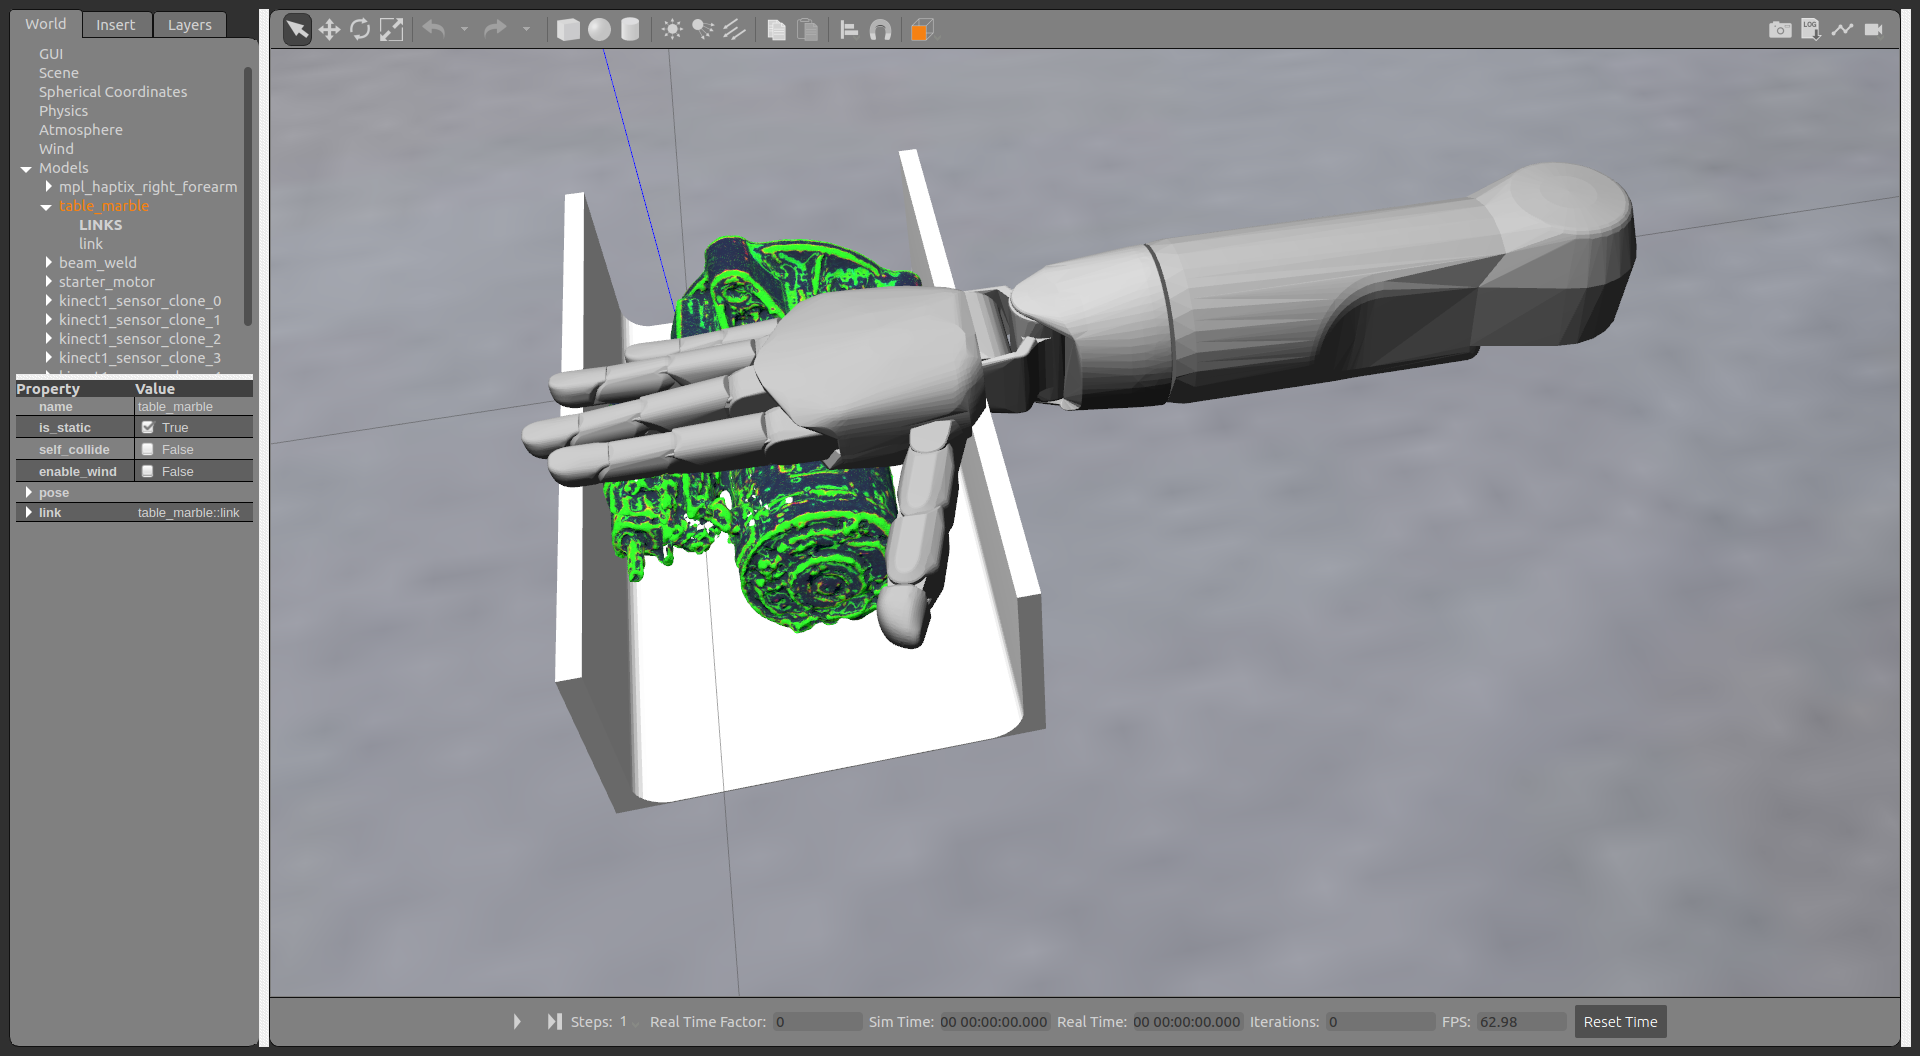
\includegraphics[height=.32\textheight]{world_1}
			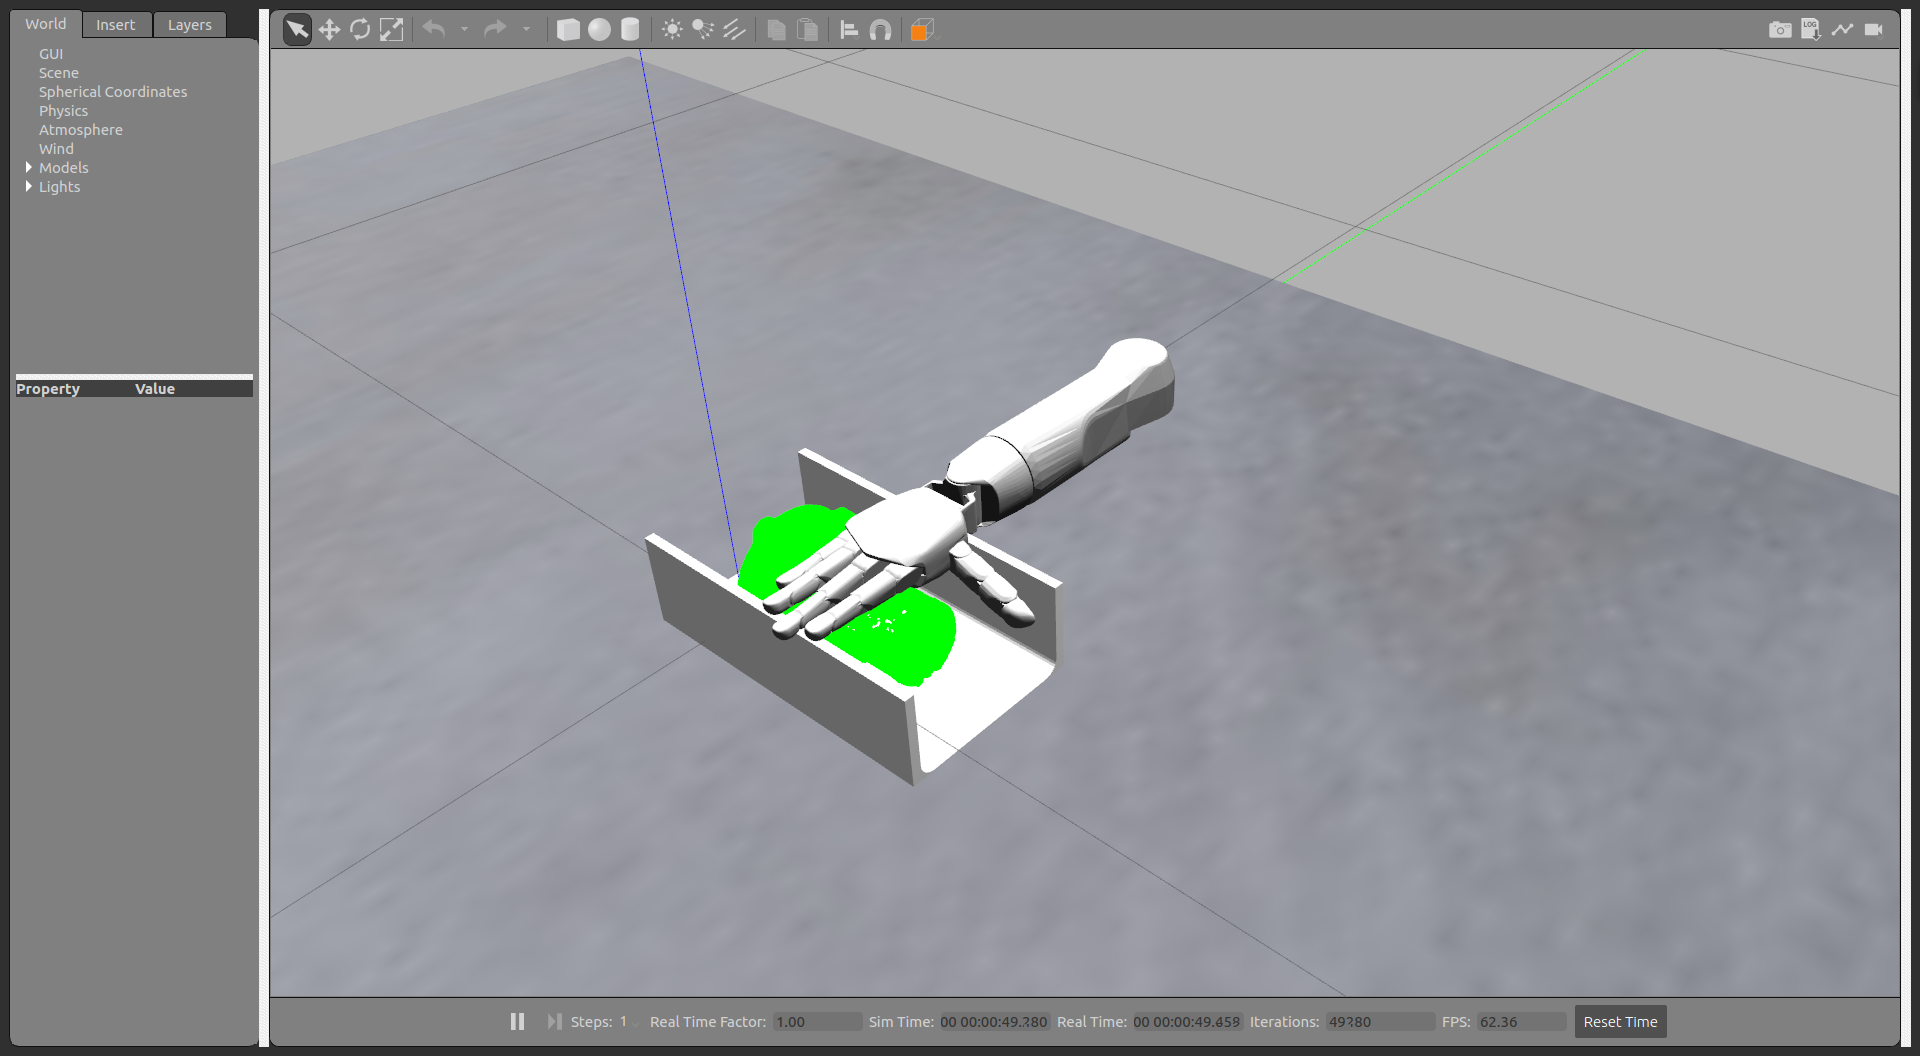
\includegraphics[height=.32\textheight]{world_9}
		\end{figure}
	\end{itemize}
\end{frame}


\section{\scshape 3D objects}
\subsection*{3D objects}
\begin{frame}{3D objects}
	\begin{itemize}
		\item 3D objects representation
		\begin{itemize}
			\item Mesh for 3D rendering
			\item Point cloud for depth sensor analysis
			\item Color segmentation for separating target objects from background
		\end{itemize}
		\begin{figure}[!ht]
			\centering
			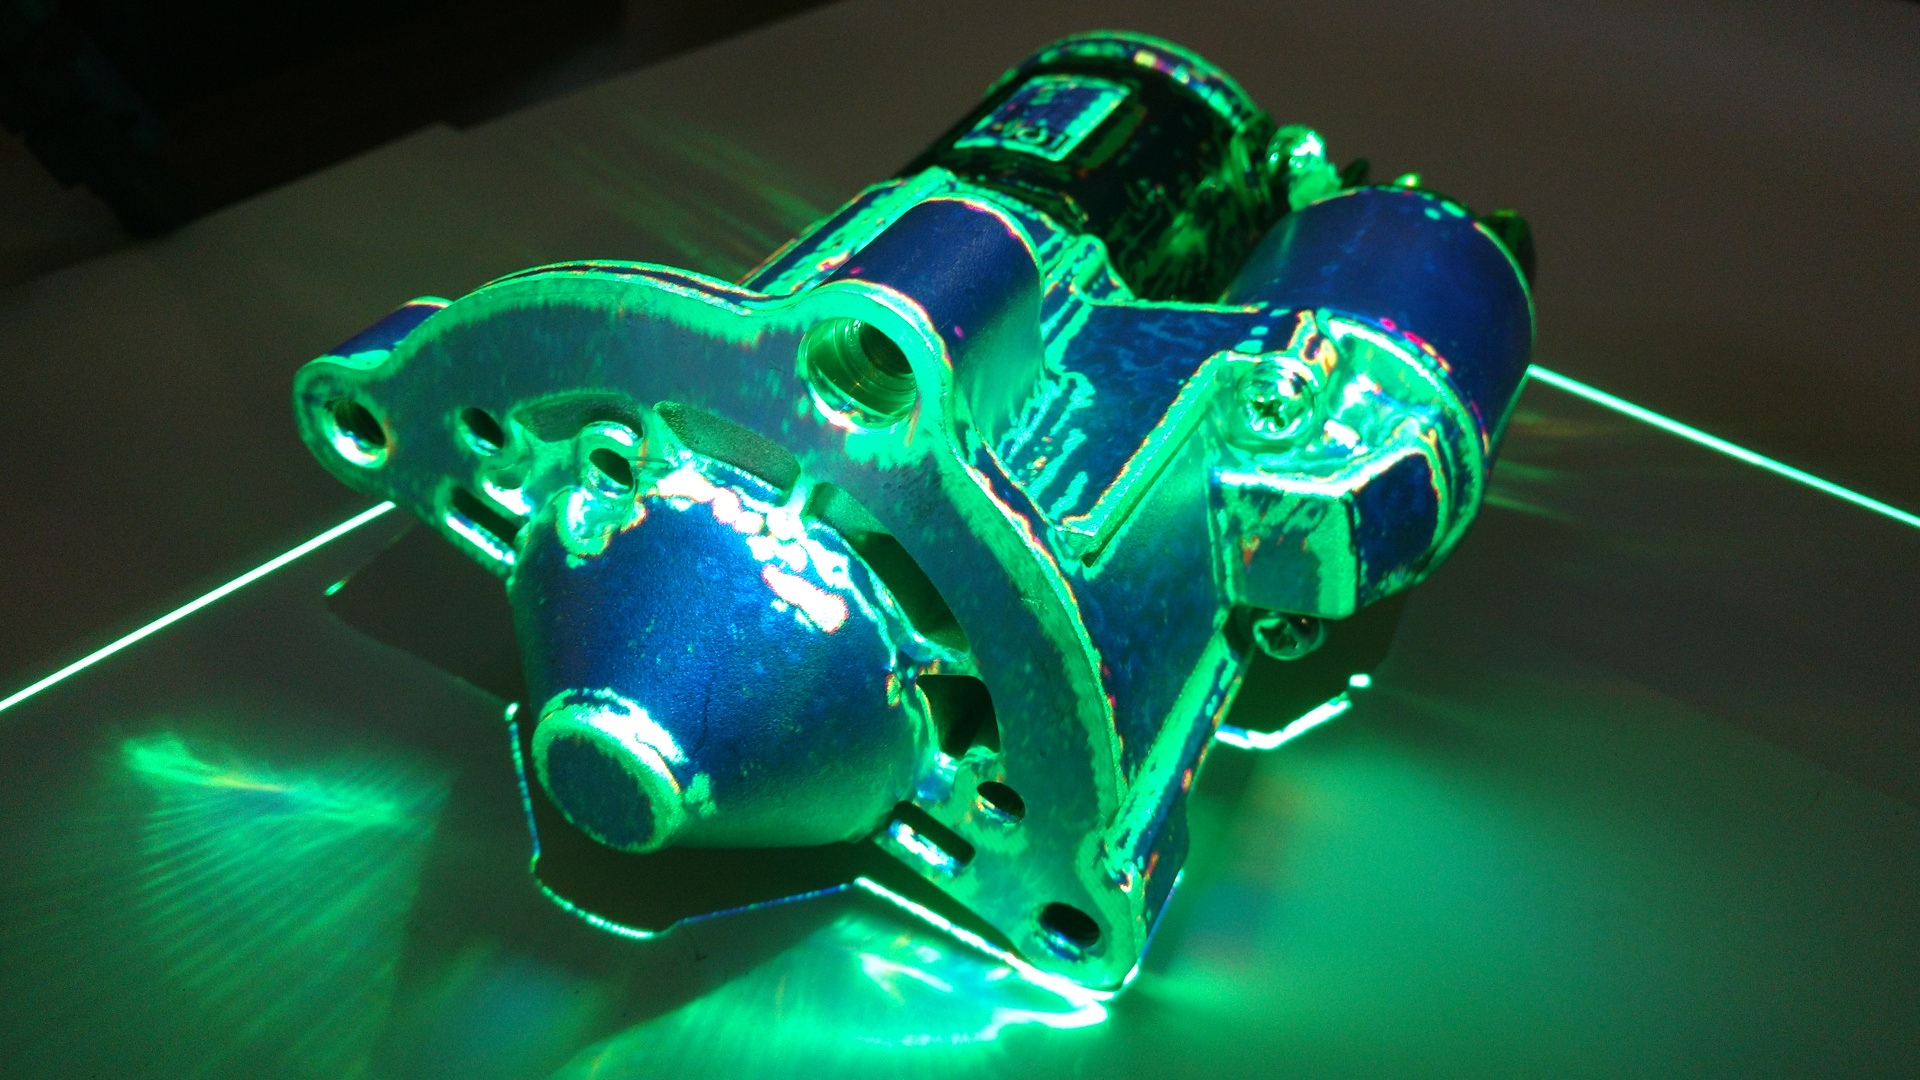
\includegraphics[height=.32\textheight]{projection-mapping}
			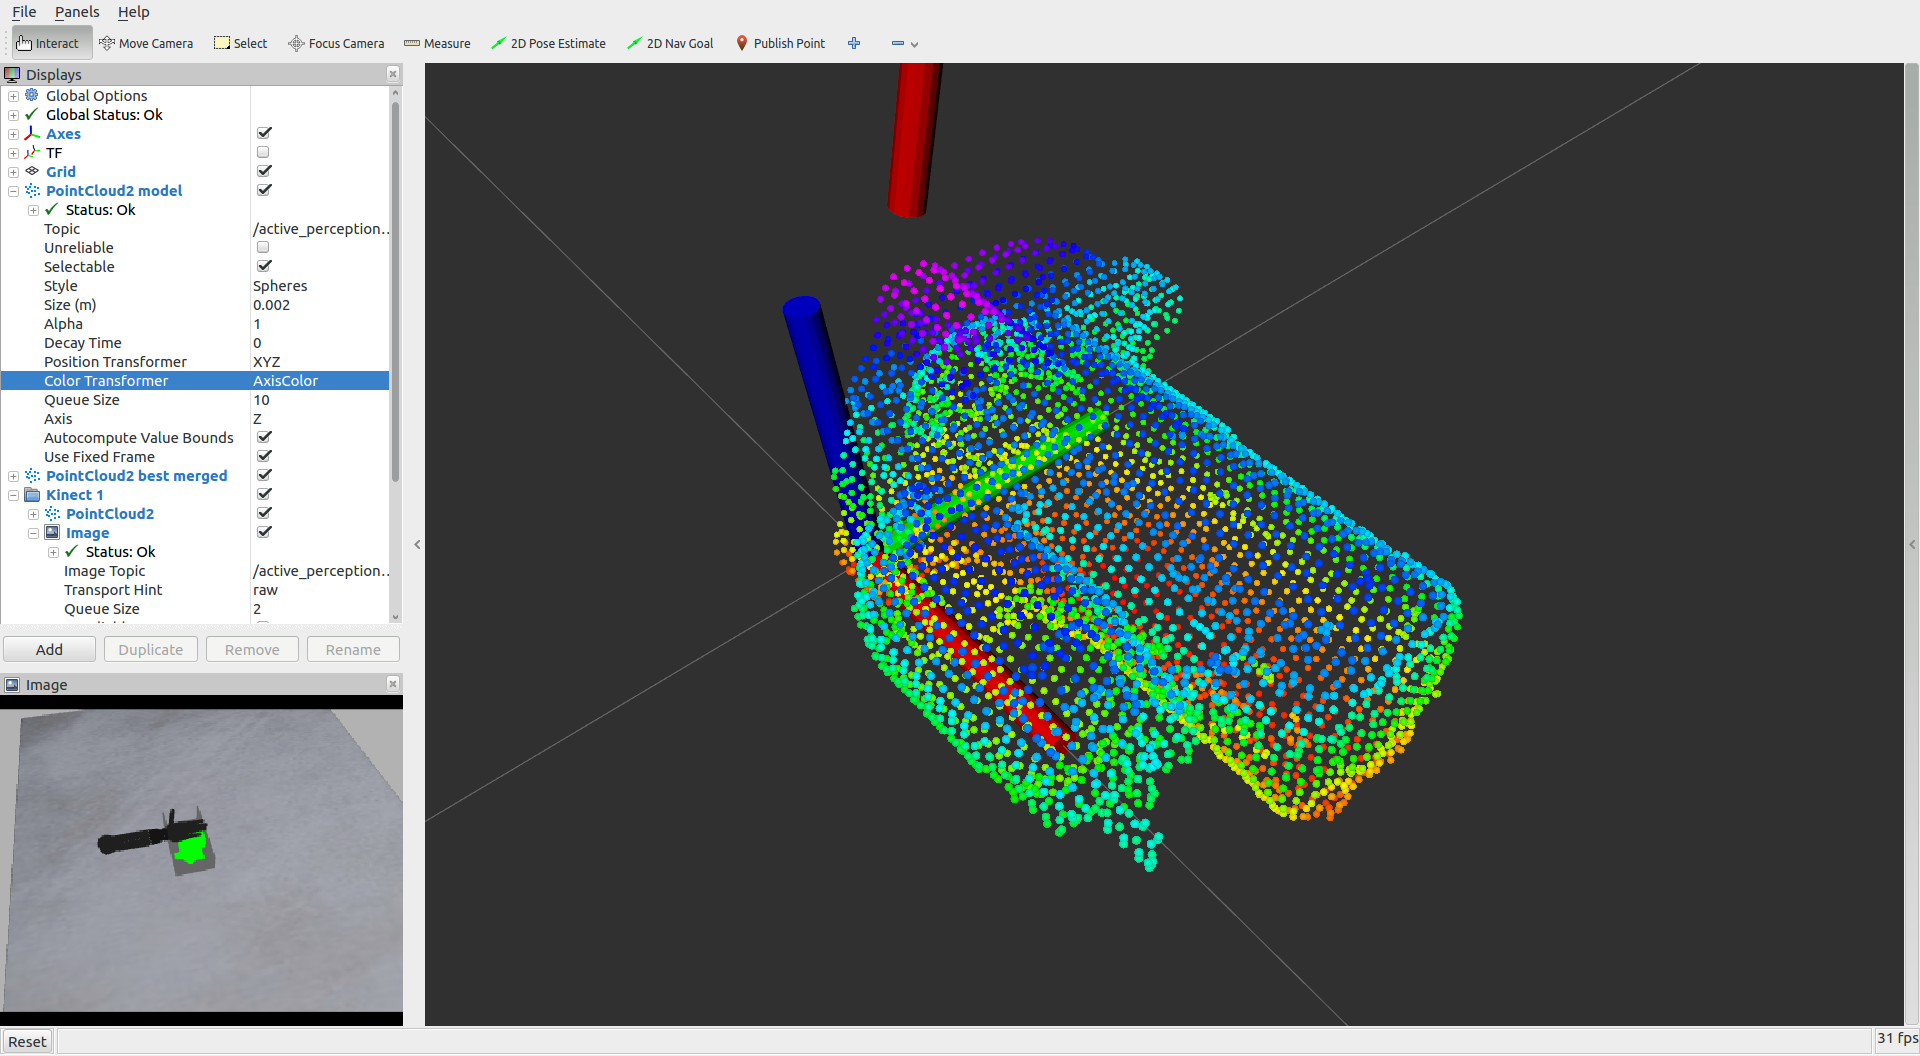
\includegraphics[height=.32\textheight]{rviz_4}
		\end{figure}
	\end{itemize}
\end{frame}


\section{\scshape 3D sensing}
\subsection*{3D sensing}
\begin{frame}{3D sensing}
		\begin{itemize}
			\item Modeling of several types of 3D depth sensors
			\begin{itemize}
				\item Sensors resolution
				\item Sensors field of view
				\item Range of measurements
			\end{itemize}
			\item Uniform or random disposition within a given set of regions of interest
			\begin{figure}[!ht]
				\centering
				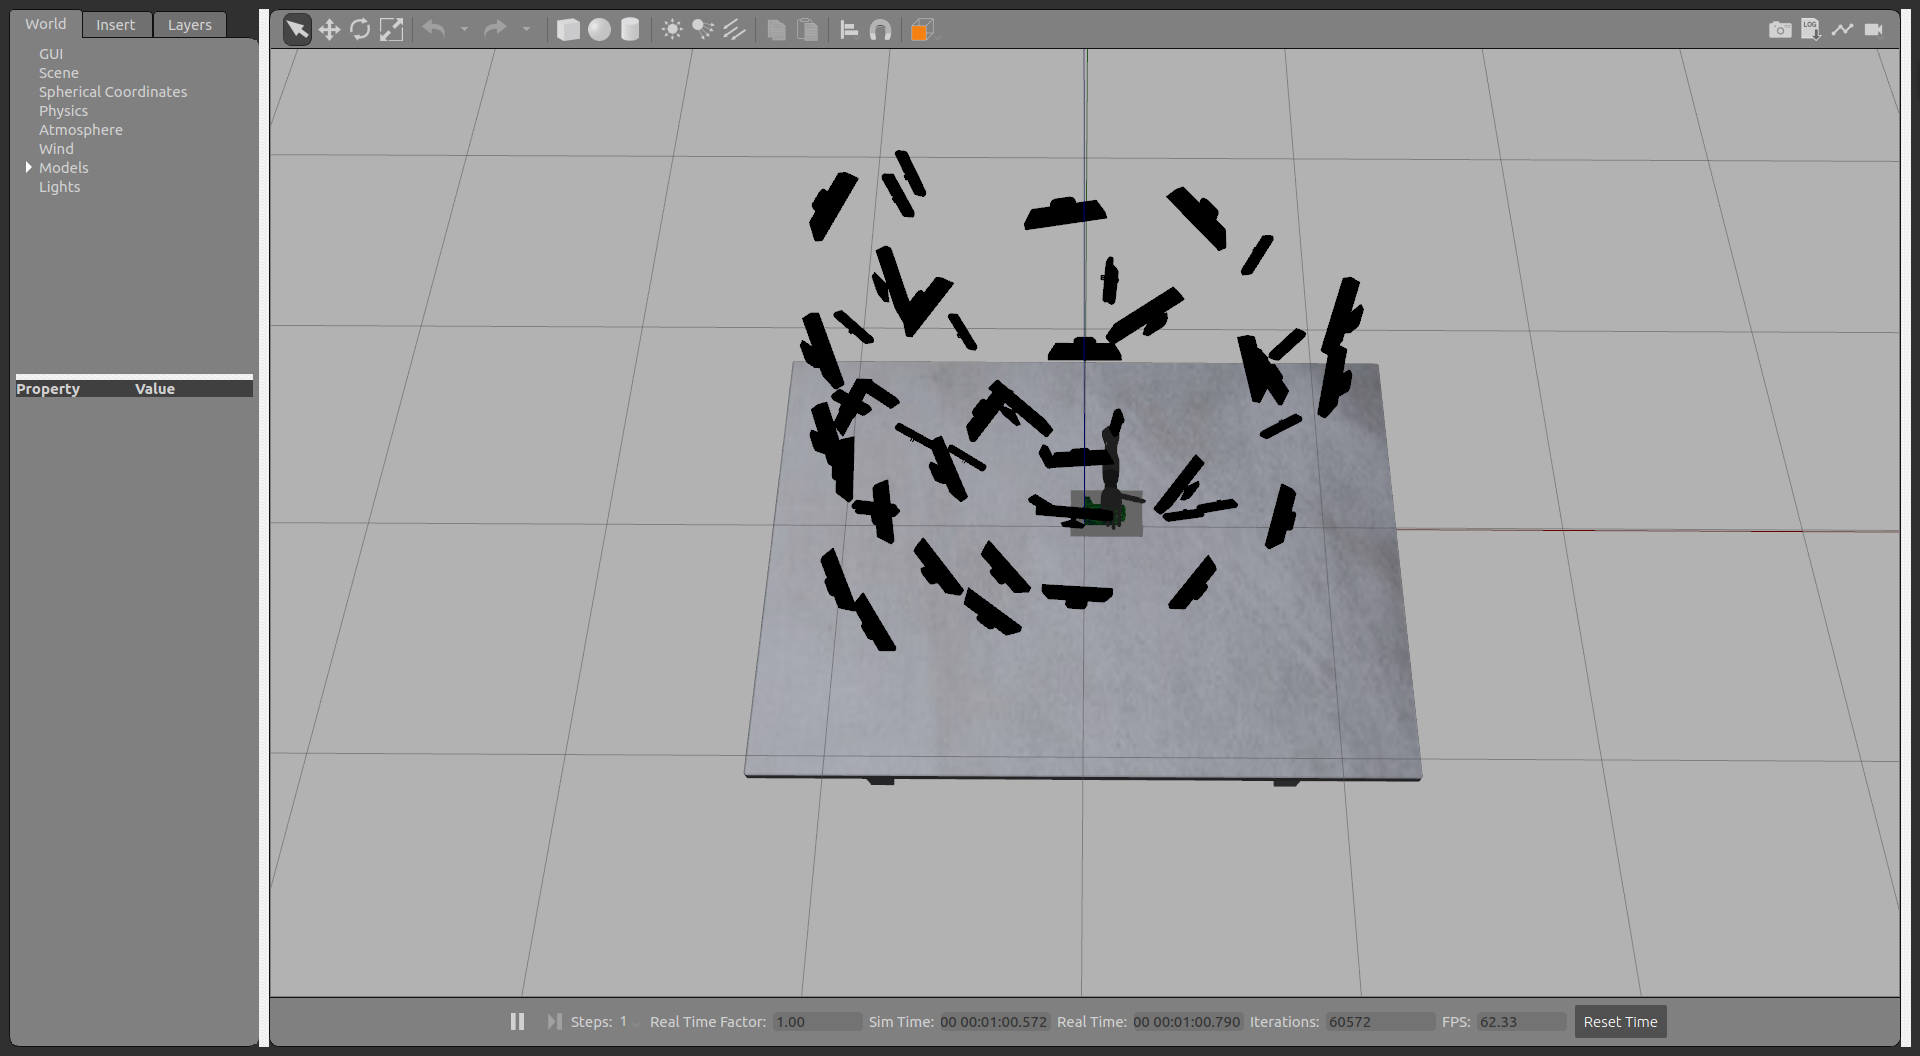
\includegraphics[height=.32\textheight]{world_2}
				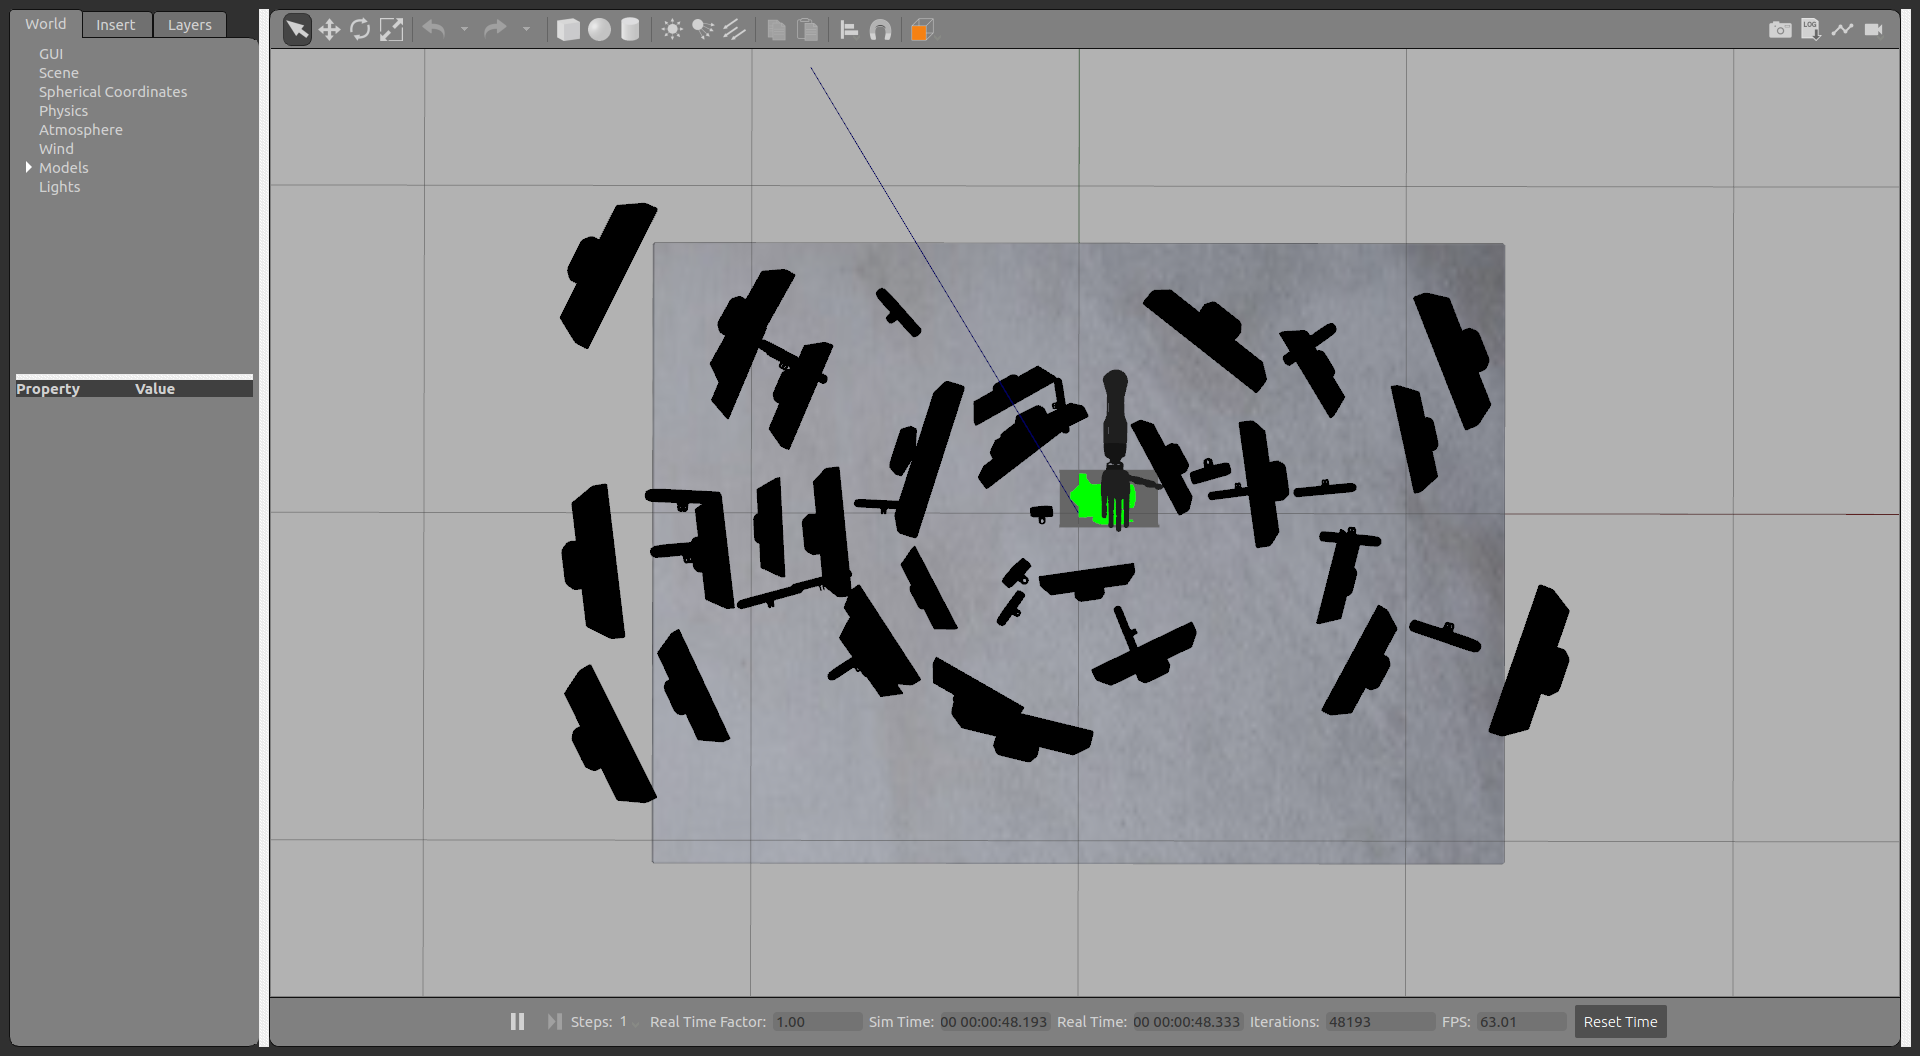
\includegraphics[height=.32\textheight]{world_6}
			\end{figure}
		\end{itemize}
\end{frame}

\begin{frame}{Estimation of the best sensor configuration}
	\begin{itemize}
		\item Given a set of observation positions
		\begin{itemize}
			\item If only one sensor is available
			\begin{itemize}
				\item Analyze all sensors data from each observation position
				\item Apply a voxel grid space partition to avoid reduce variability of the estimated surface area observed by each sensor
				\item Choose the sensor that can observe the most surface area of the objects
			\end{itemize}
		\end{itemize}
		\begin{figure}[!ht]
			\centering
			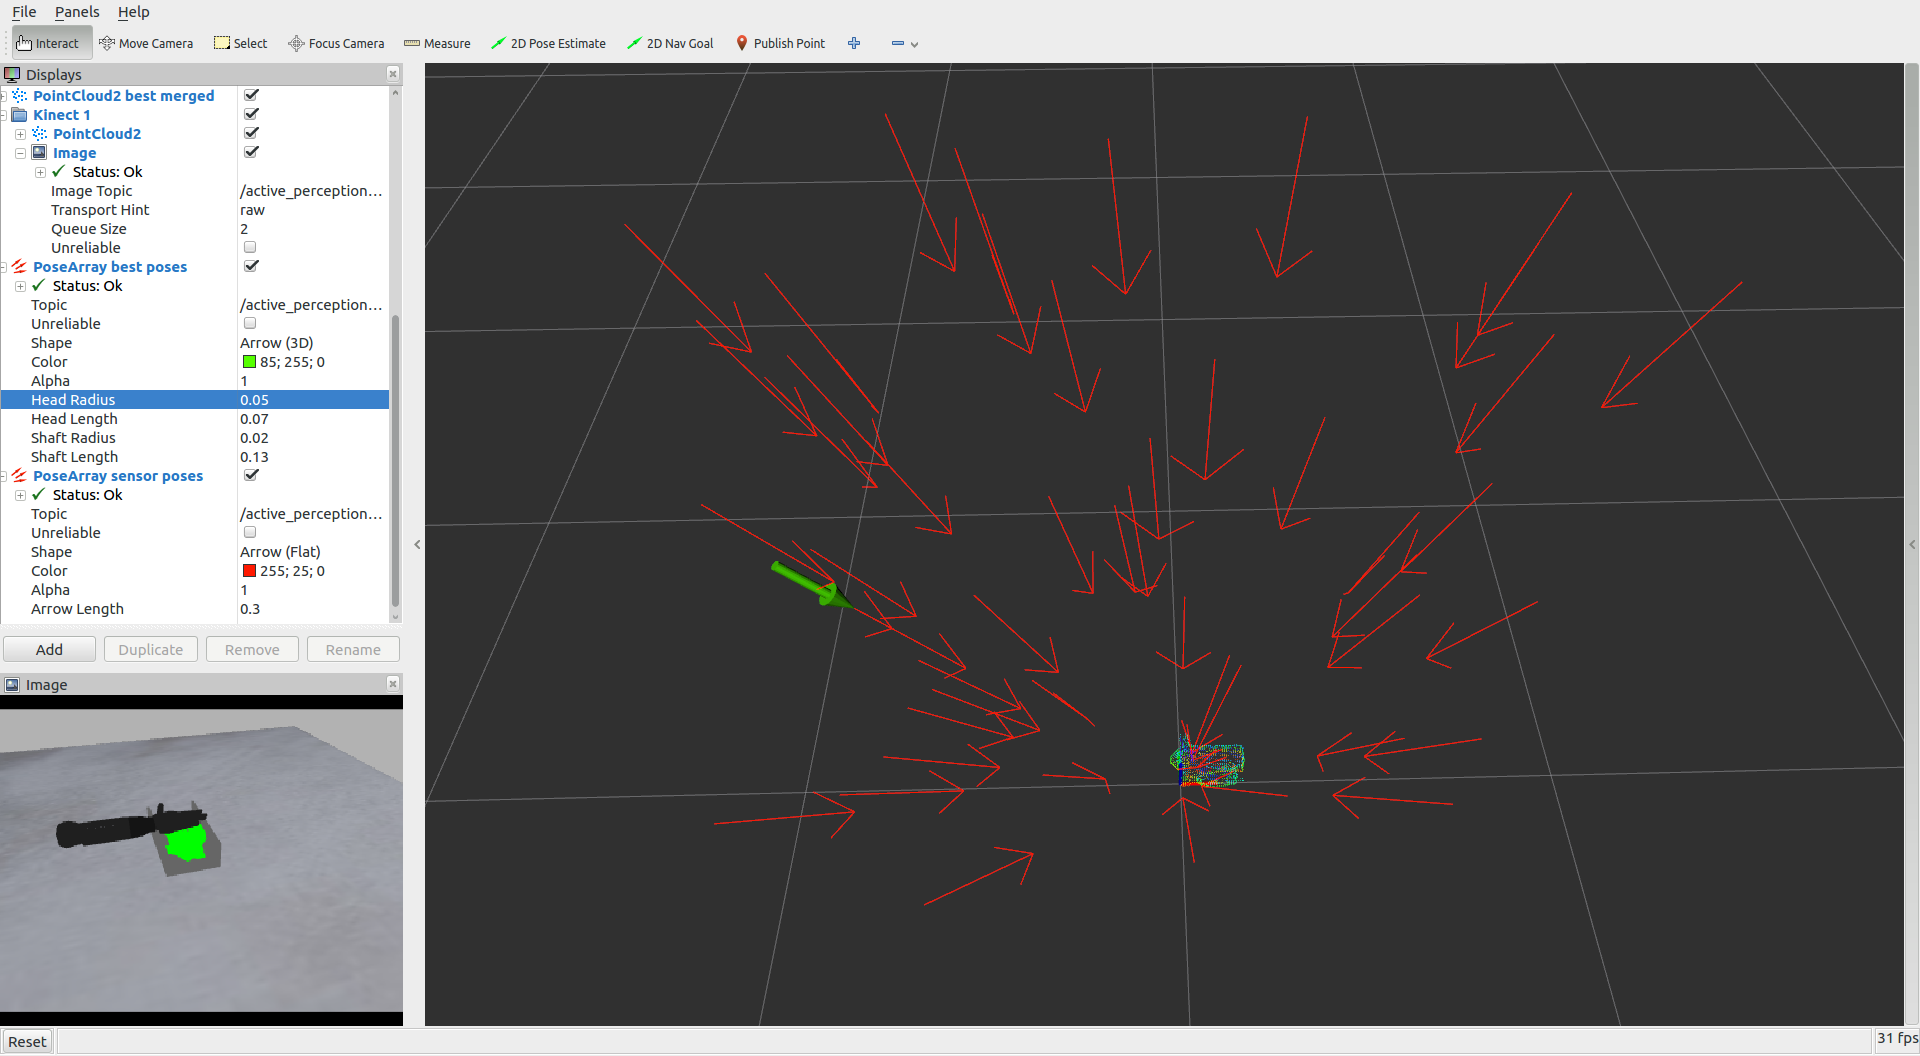
\includegraphics[height=.32\textheight]{rviz_6_1_sensor}
		\end{figure}
	\end{itemize}
\end{frame}

\begin{frame}{Estimation of the best sensor configuration}
	\begin{itemize}
		\item Given a set of observation positions
		\begin{itemize}
			\item If several sensors area available (type and quantity adjustable)
			\begin{itemize}
				\item Extract point clouds for each observation point
				\item Using a RANSAC approach, choose randomly a set a N sensors
				\item Merge the sensor data and estimate the observable surface area
				\item At the end of a given number of iterations or if the observable area reaches a given minimum, terminate the search, keeping the best sensor configuration found
			\end{itemize}
		\end{itemize}
		\begin{figure}[!ht]
			\centering
			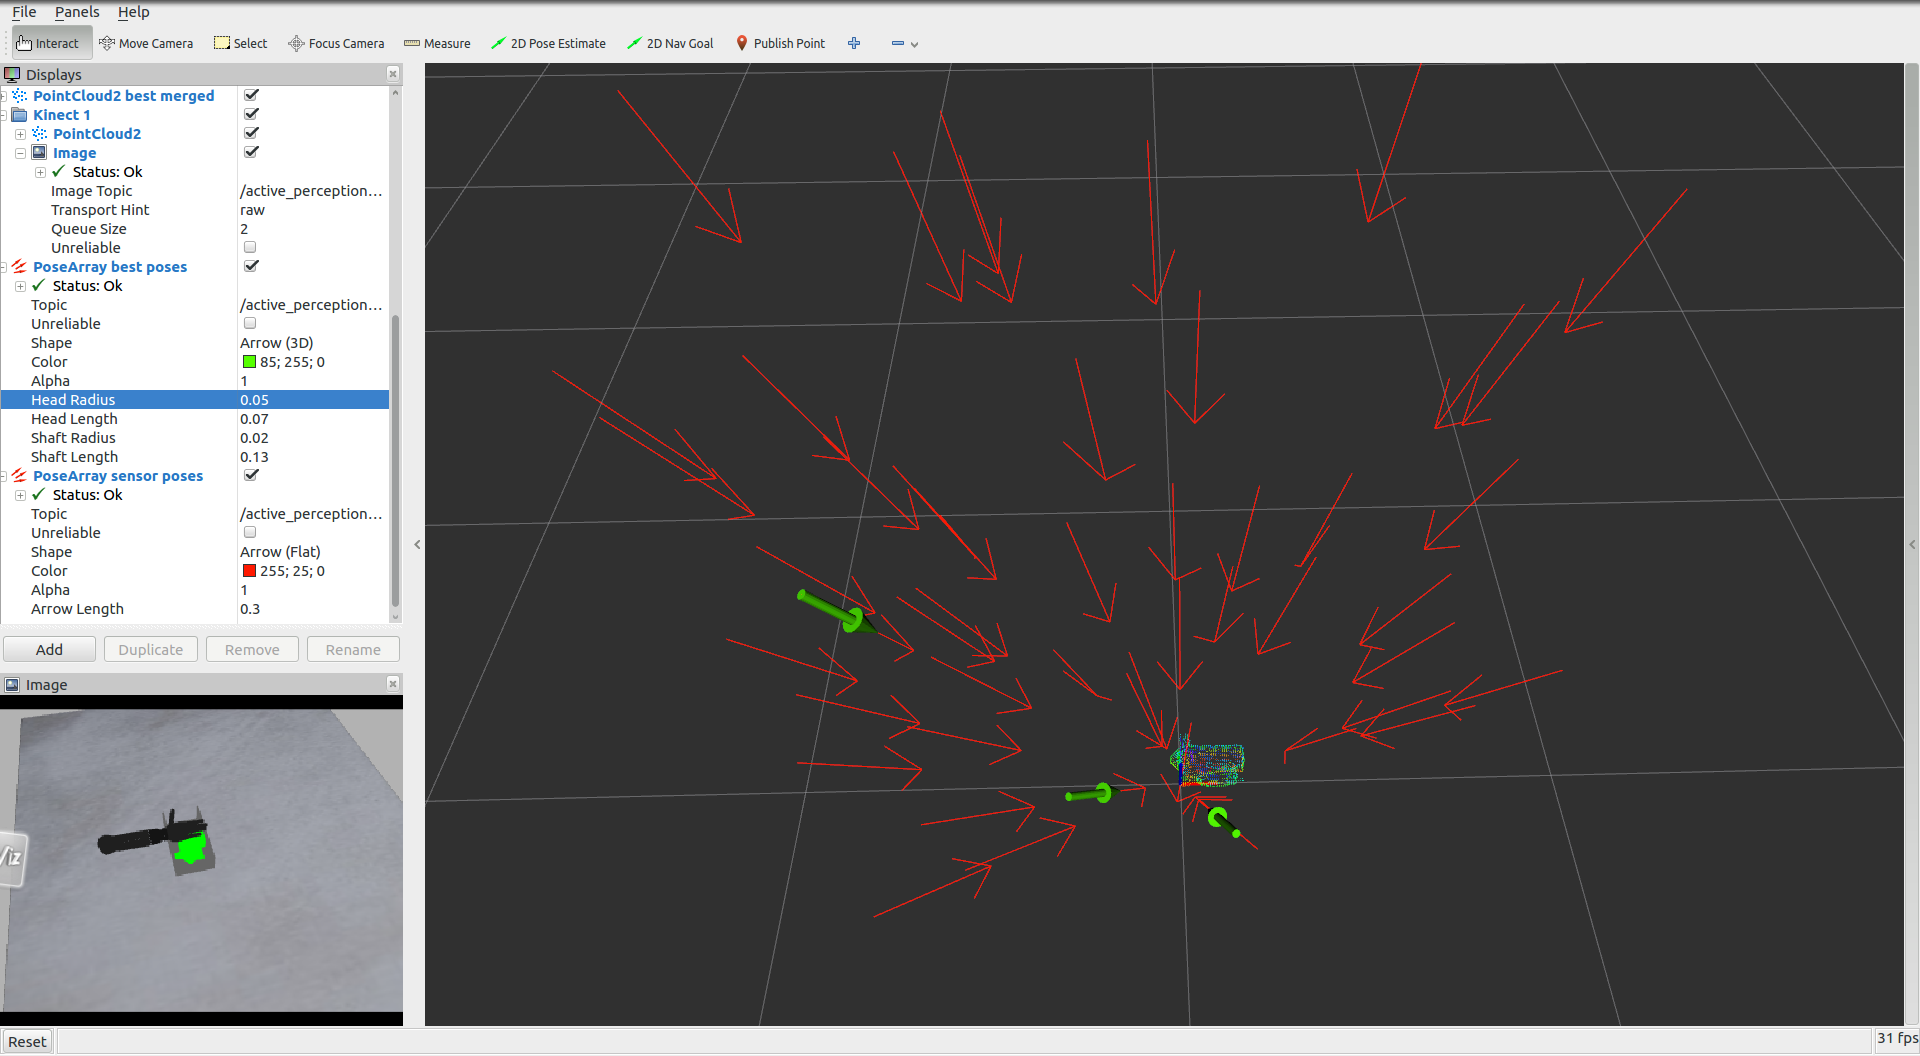
\includegraphics[height=.32\textheight]{rviz_6}
		\end{figure}
	\end{itemize}
\end{frame}
